\documentclass{article}
\title{Nechyba Ch.18 弹性、价格扭曲政策与非价格配给}
\author{Dawei Wang}
\date{\today}
\usepackage{ctex}
\usepackage{amsmath}
\usepackage{amssymb}
\usepackage{graphicx} %插入图片的宏包
\usepackage{float} %设置图片浮动位置的宏包
\usepackage{subfigure} %插入多图时用子图显示的宏包
\begin{document}
	\maketitle
	在一个以稀缺性定义的世界里,价格代表着对稀缺资源配给(ration)的一种方式,该方式决定哪个消费者消费哪种商品,每个人工作多少,现在以及未来的消费量是多少,每个人面对的风险是多大。
	
	总有某种机制能够决定谁可以获得商品而谁不可以。市场价格代表这样的一种配给机制,当我们加上其他一些制度以提高市场机制的效率,我们会不自觉地掺入其他配给机制。
	
	价格扭曲的影响大小取决于贤妃这和生产者对价格变化的反应程度,也就是消费者或生产者行为的弹性(elasticity)。
	
\section{市场与价格扭曲政策的相互作用}

对完全竞争市场的两种主要的政策进行分析:1.以降低价格以使消费者收益为目标;2.以提高价格以使生产者收益为目标。

\subsection{弹性与剩余的分割}

\begin{figure}[H] %H为当前位置,!htb为忽略美学标准,htbp为浮动图形
	\centering %图片居中
	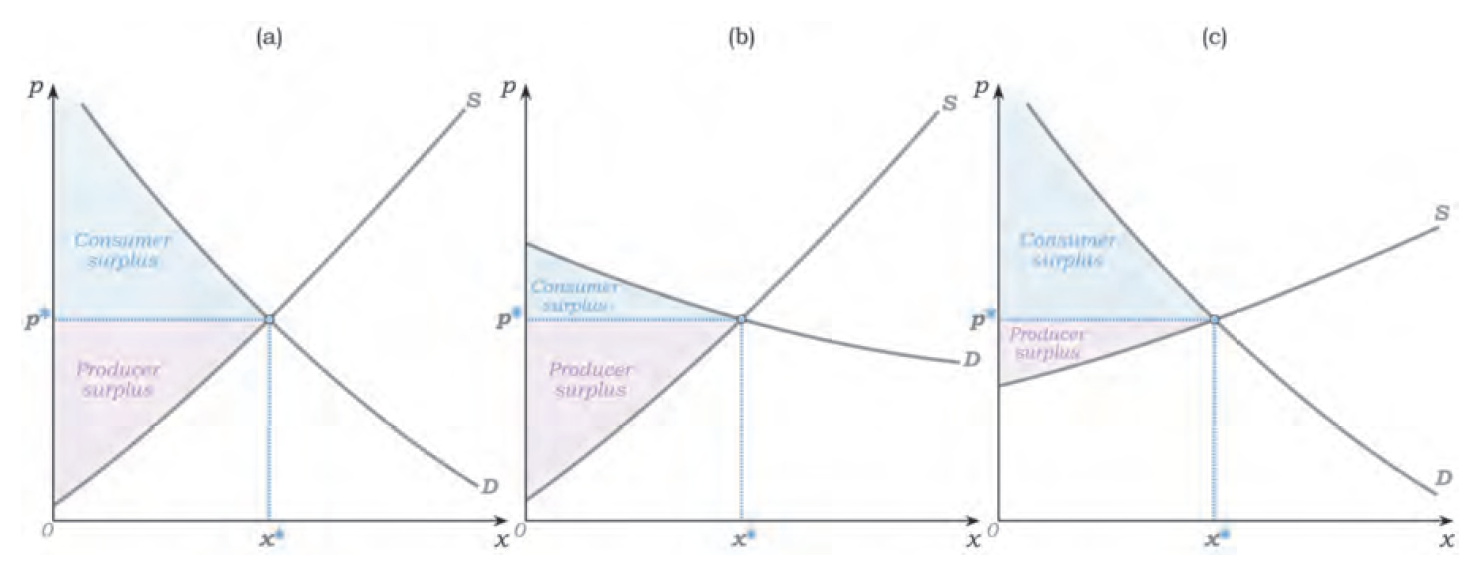
\includegraphics[width=1\textwidth]{18_1} %插入图片,[]中设置图片大小,{}中是图片文件名
	\caption{Different Distributions of Consumer and Producer Surplus in a Market} %最终文档中希望显示的图片标题
	\label{Fig.main2} %用于文内引用的标签
\end{figure}

上图表明,社会剩余在消费者和生产者之间的分配取决于需求曲线和供给曲线的相对斜率。这是正确的,不过经济学家使用“价格弹性”这一概念来完善这一描述。

使用斜率进行描述的问题在于曲线的斜率取决于横轴与纵轴的计量单位。弹性的引入,使得行为的变化从绝对值的变化转变成了百分比的变化。弹性就是指行为对价格变化的反应程度。

\begin{figure}[H] %H为当前位置,!htb为忽略美学标准,htbp为浮动图形
	\centering %图片居中
	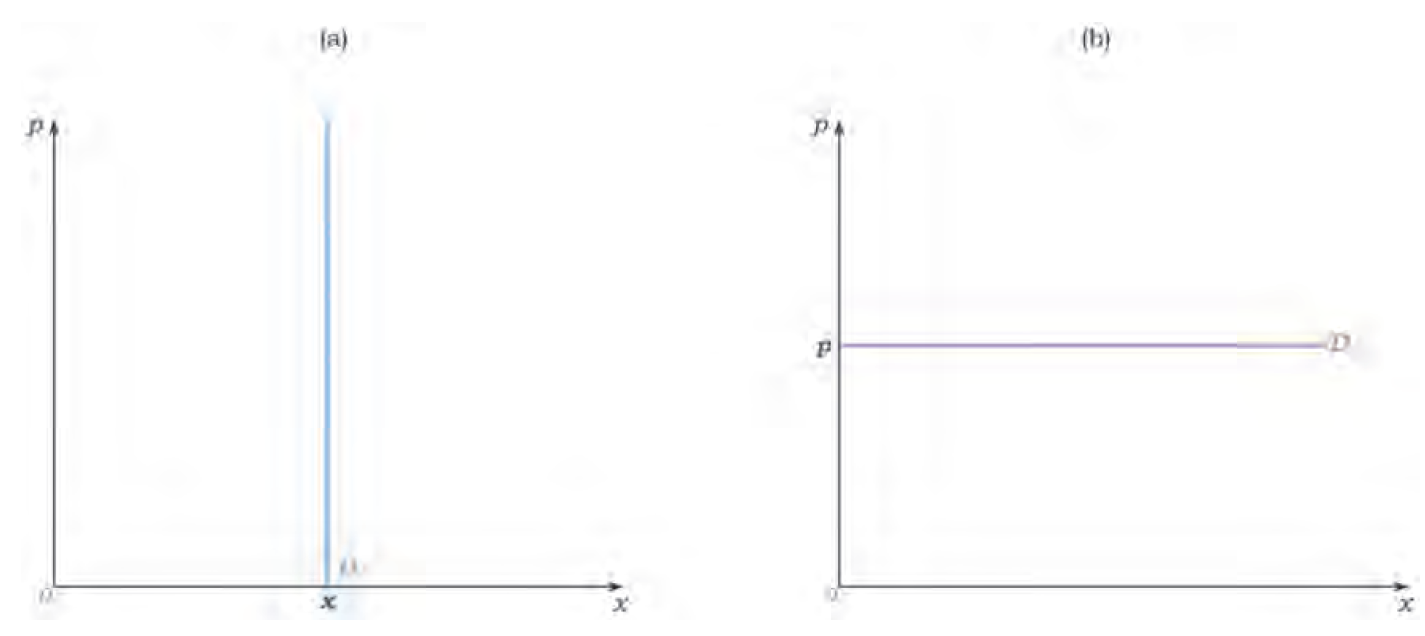
\includegraphics[width=1\textwidth]{18_2} %插入图片,[]中设置图片大小,{}中是图片文件名
	\caption{Perfectly Price Inelastic and Elastic Demand} %最终文档中希望显示的图片标题
	\label{Fig.main3} %用于文内引用的标签
\end{figure}

\hspace*{\fill}

价格弹性和消费支出

当商品的价格上涨或是下降时,一个消费者时增加还是减少在某一种特定商品上的消费取决于ta对价格变化的反应程度。意即价格变化对消费者支出的影响由需求价格弹性来决定。

\begin{figure}[H] %H为当前位置,!htb为忽略美学标准,htbp为浮动图形
	\centering %图片居中
	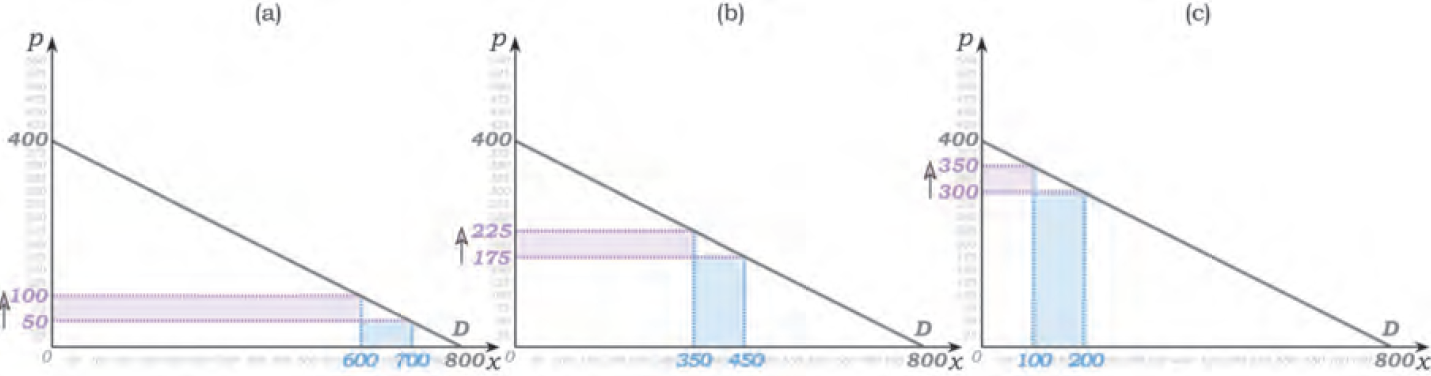
\includegraphics[width=1\textwidth]{18_3} %插入图片,[]中设置图片大小,{}中是图片文件名
	\caption{Price Elasticity and Changes in Consumer Spending} %最终文档中希望显示的图片标题
	\label{Fig.main4} %用于文内引用的标签
\end{figure}

若价格弹性小于0大于-1,价格上涨会造成消费者开支增加;若价格弹性为-1,价格上涨对消费者开支没有影响;若价格弹性小于-1,价格上涨会导致消费者开支下降。

当需求价格弹性是大于-1小于0,需求对价格变化相对无弹性或者说反应相对不敏感;当需求价格弹性低于-1时,需求对价格变化相对有弹性或者说反应敏感。

\hspace*{\fill}

生产者的价格弹性是正数(当商品不是吉芬品),因为价格上涨会促使生产者生产更多。

\subsection{价格下限}

价格下限是在一个特定的市场中政府授权的最低法定价格。低于这个价格下限的交易是非法的。价格下限如果低于均衡价格,则不会对这个市场由任何影响。因为市场会自动设置一个价格下限以上的价格,而买家和卖家以这个市场交易。

实行一个高于均衡价格的价格下限,会出现商品过剩(surplus)。除非出现一种非价格配给(non-price rationing)机制,将产品分配给那些需求量比价格下限处的需求量少的消费者。因此价格下限导致市场进入不均衡(disequilibrium)状态。

\begin{figure}[H] %H为当前位置,!htb为忽略美学标准,htbp为浮动图形
	\centering %图片居中
	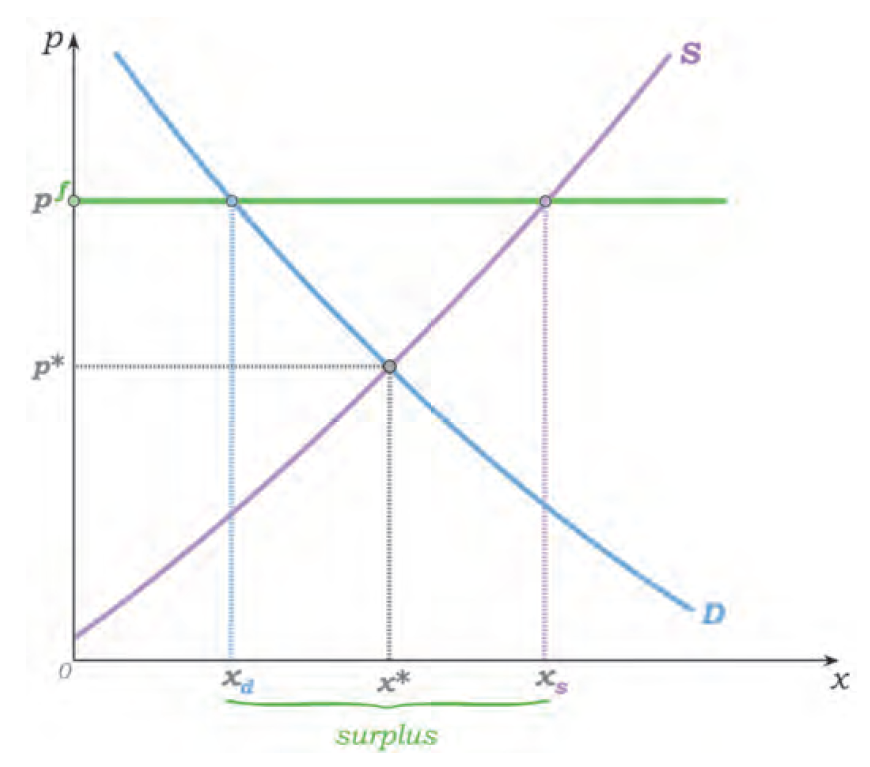
\includegraphics[width=1\textwidth]{18_4} %插入图片,[]中设置图片大小,{}中是图片文件名
	\caption{Disequilibrium Caused by a Price Floor} %最终文档中希望显示的图片标题
	\label{Fig.main5} %用于文内引用的标签
\end{figure}

虽然政府设定了高于均衡价格的价格下限但是供应商不可能一直超出销售额地生产。因此,除非出现某种非价格配给机制来再次确保需求量等于供给量,经济才能再次达到均衡状态。这种非价格配给机制一方面可能由政府来实现——在意识到这种由设定价格下限产生的问题后,政府会制定相应的政策;另一方面也可能与政府干预无关,而由一些其他形式地非价格配给机制造成,这些机制有使市场重新达到均衡的趋势。

\hspace*{\fill}

有价格下限的市场中的非价格配给

考虑政府没有明确想解决价格下限造成的不均衡问题的情况。在实行价格下限的情况下,若每个个体生产者都知道所有的生产者在试图卖出超出消费者需求的更多商品,ta们愿意付出额外的努力来试图说服消费者选择自己的商品。生产者这种额外的努力也是额外的成本无论是积极宣传还是游说政府给予特殊优势从而促使消费者选择某一家而非另一家生产者的商品。因此,无论采取何种形式的努力,生产者的MC和AC曲线将向上移动,这反过来又导致市场供给曲线向上移动,直到它与市场需求曲线在数量为$ x_d $处相交。如果最初市场上生产者面临着不同的成本曲线,那些成本较低的生产者最容易通过付出额外成本来吸引消费者,而其他生产者这样做可能会退出市场。

\begin{figure}[H] %H为当前位置,!htb为忽略美学标准,htbp为浮动图形
	\centering %图片居中
	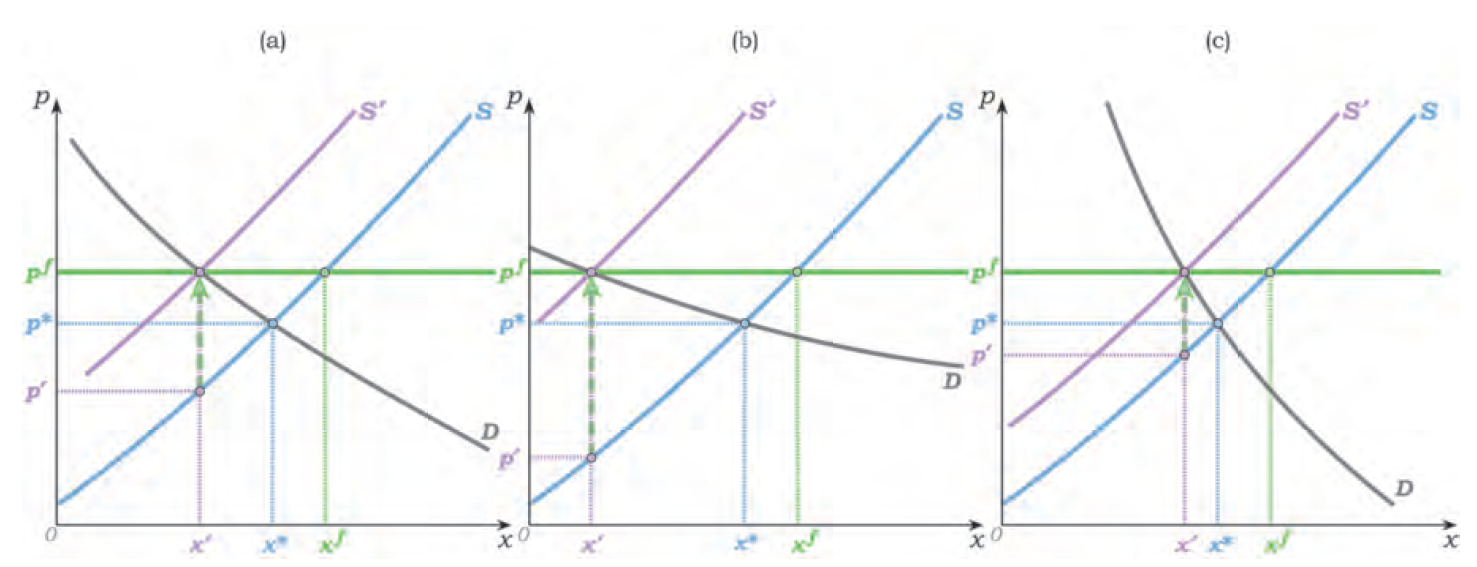
\includegraphics[width=1\textwidth]{18_5} %插入图片,[]中设置图片大小,{}中是图片文件名
	\caption{Restoring Equilibrium through Increased Costs for Producers} %最终文档中希望显示的图片标题
	\label{Fig.main6} %用于文内引用的标签
\end{figure}

当心的均衡出现,成本上升程度为$ (p^f-p') $。这是一个新的均衡,因为需求再一次等于供给,生产者和消费者也再一次通过自己的努力使自己在限定的条件下达到最优。意即消费者根据自己的预算限制来决定消费量,此时他们的边际支付意愿等于新的价格(或者,他们得到不再购买x的角点解),而生产者选择的生产量就是新的价格与其新MC的交点处的生产量(或者他们一起推出市场)。

市场产出的减少,不仅取决于政府制定了多高的价格下限,也取决于需求的价格弹性。需求的价格弹性大,则均衡的产出下降多,反之反是。

\hspace*{\fill}

价格下限下政府的非价格配给

政府在意识到价格下限将导致市场产出的减少后,将实行其他政策来抵消价格下限所产生的市场反应。例如常见的“农产品价格支持”政策,政府设定某些农产品的价格下限,同时承诺购买所有由于价格下限所导致的农产品剩余。

实行这类政策时,生产者没有动机再努力吸引消费者,因为卖不出去的农产品都将有政府以价格$ p^f $收购。因此,市场供给曲线不会变动。

\hspace*{\fill}

福利的变化和价格下限DWL的产生

\begin{figure}[H] %H为当前位置,!htb为忽略美学标准,htbp为浮动图形
	\centering %图片居中
	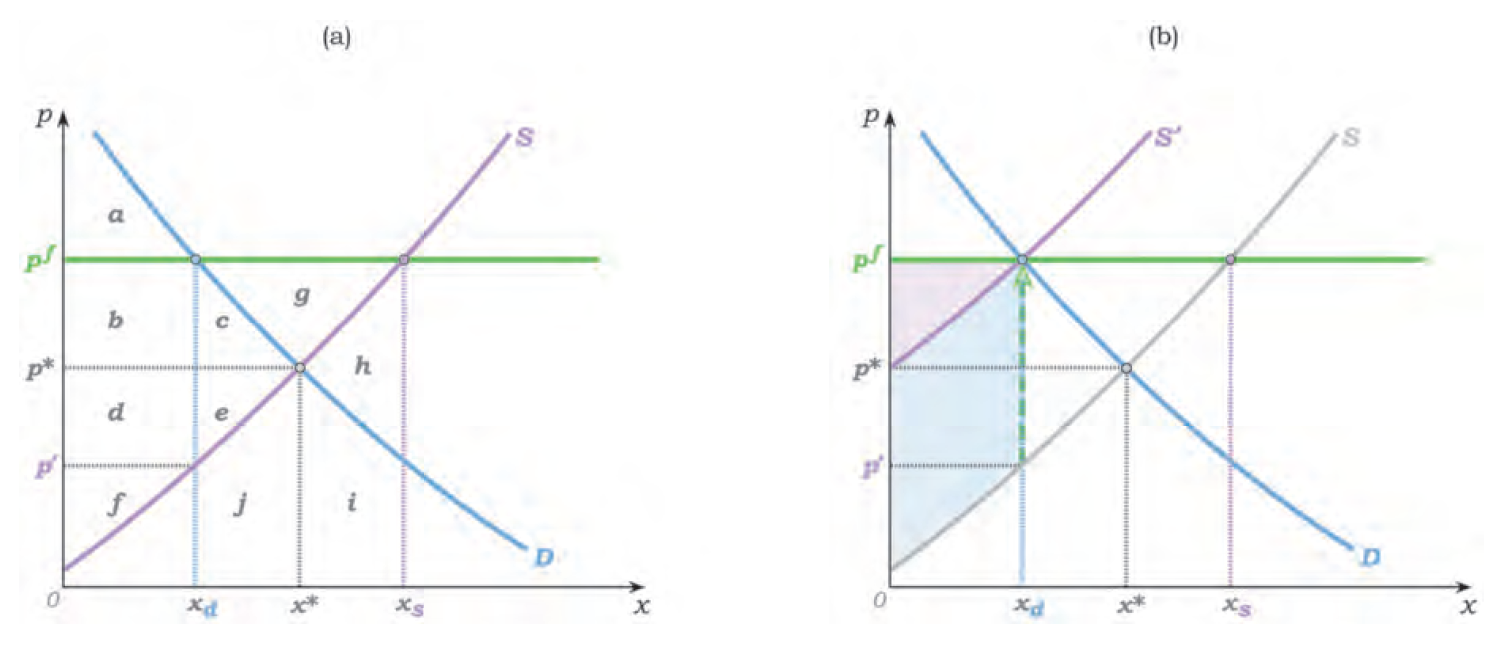
\includegraphics[width=1\textwidth]{18_6} %插入图片,[]中设置图片大小,{}中是图片文件名
	\caption{Changes in Costs and Surplus when Price Floors Are Imposed} %最终文档中希望显示的图片标题
	\label{Fig.main7} %用于文内引用的标签
\end{figure}

没有实行价格下限时,市场均衡价格为$ p^* $,生产量为$ x^* $时的消费者剩余为$ (a+b+c) $,生产者剩余为$ (d+e+f) $。

考虑政府实行价格下限而不辅以其他政策时的新均衡,由于生产者需要多加努力以吸引消费者造成成本增加,供给曲线上移。


消费者剩余为$ (a) $,供给的变动是由于边际成本的增加造成的$ (p^f-p') $造成的。浅灰色阴影部分代表新的生产者剩余,而深灰色部分代表着生产者增加的成本。假定区域$ (f) $等于新的生产者剩余。

消费者和生产者总剩余从之前的$ (a+b+c+d+e+f) $缩减为$ (a+f) $。生产者成本增加——$ (b+d) $区域的大小由于生产者面对的具体成本类型决定。比如,成本可以用在向消费者投放广告上,但是这是一种社会性浪费。广告是一种使消费者从信息中受益的生产者利益的转移。区域$ (c+e) $就是明确的损失。因此实行价格下限出现的新均衡所带来的DWL至少是区域$ (c+e) $,有时候可以达到区域$ (b+c+d+e) $。

考虑政府实行价格下限并辅以政府购买政策来冲抵价格下限造成的非均衡时的新均衡。市场中的消费者只会购买$ x_d $,消费者剩余为区域$ (a) $。生产者生产$ x_s $,而价格$ x_s $与$ x_d $之间的差额由政府购买,因此生产者所有的产品都可售罄。新的生产者剩余为价格下限之下供给曲线S之上的部分,增加为$ (b+c+d+e+f+g) $。同时政府购买支出也是一种社会成本。政府以$ p^f $购买$ (x_s-x_d) $,总成本为$ p^f(x_s-x_d) $,表示在图中就是$ (c+e+g+h+i+j) $的矩形。消费者剩余减去生产者总剩余减去政府购买的升本就是$ (a+b+d+f-h-i-j) $。

因此实行价格下限之前的总剩余就是$ (a+b+c+d+e+f) $,而实行之后总剩余变为$ (a+b+d+f-h-i-j) $——这里假设政府购买完多余商品就将之扔掉。这样,价格下限就产生了大小为$ (c+e+h+i+j) $的无谓损失。如果政府并没有扔掉购买的商品,而是把商品卖给对之估值最高的消费者,对商品估值高于$ p^f $的消费者已经在市场中购买了商品$ x_d $,而对部分商品估值最高的正是需求曲线上$ x_d $到$ x_s $之间的部分。消费者对政府购买的那部分商品的估值就是$ x_d $到$ x_s $之间低于需求曲线的部分,在图中表示就是区域$ (c+e+i+j) $。这样政府就得到$ (c+e+i+j) $大小的剩余。从无谓损失中减去此部分,就只有区域$ (h) $了。无谓损失的大小取决于政府如何把所购买的商品再次推销给消费者,而这个无谓损失可能低至区域$ (h) $,也可能高达$ (c+e+h+i+j) $。

最常见的价格下限例子就是最低工资标准。最低工资是影响劳动力市场的一种价格下限,政府要求雇佣者支付高于均衡工资的工资给劳动者,而这样的劳动市场一般都是与相对缺少技术含量的劳动挂钩。

\subsection{价格上限}

价格上限是法律上强制执行的最高价格,以任何高于此上限的价格交易都是违法的。价格上限若高于均衡价格,则对市场毫无影响,因为市场作用形成的均衡价格本来就低于价格上限。因此,只有当价格上限低于均衡价格时才有效力。

\begin{figure}[H] %H为当前位置,!htb为忽略美学标准,htbp为浮动图形
	\centering %图片居中
	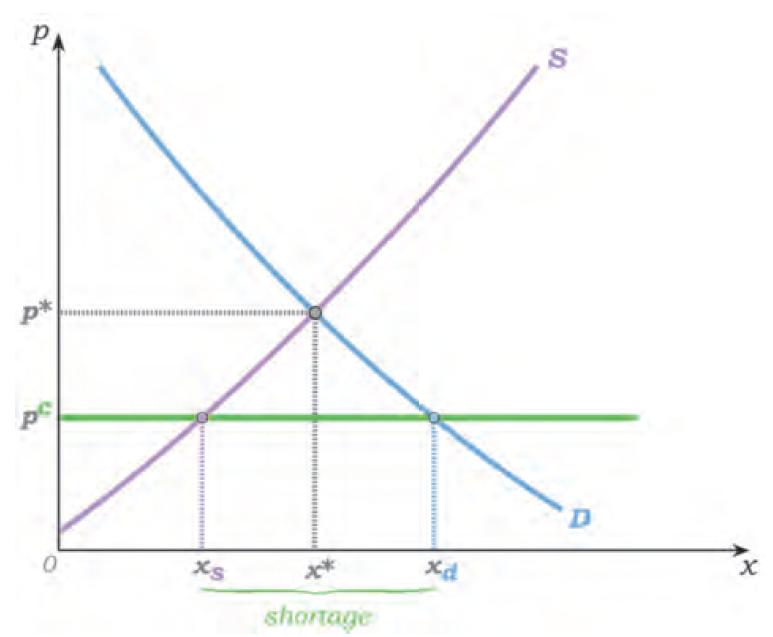
\includegraphics[width=1\textwidth]{18_7} %插入图片,[]中设置图片大小,{}中是图片文件名
	\caption{Disequilibrium when Price Ceilings Are Imposed} %最终文档中希望显示的图片标题
	\label{Fig.main8} %用于文内引用的标签
\end{figure}

价格上限的设定使得最初的均衡价格$ p^* $变得非法,由此迫使生产者与消费者以合法的最高价格$ p^c $交易。但是在这个价格上,市场上的生产者只愿意生产$ x_s $产品,市场上产生短缺(shortage)而消费者的需求有$ (x_d-x_s) $得不到满足。于是市场也因供不应求而处于非均衡状态。

若是非均衡造成商品不足,某些形式的非价格配给将取代市场价格配给的地位来将现有的商品分配给消费者。

\hspace*{\fill}

价格上限下的非价格配给

价格上限产生短缺的情况,由于产品供不应求,想要得到商品的消费者必须付出额外的努力才可以得到。这些额外的努力是消费者必须付出的成本,因此,消费者对每单位产品的边际支付意愿都降低。这意味着,需求曲线将下降,因为消费者需要把付出的额外努力的成本考虑进去以获得生产数量受限的产品。这些努力可能有多种形式,例如排队,或者被列入候选者名单,甚至是贿赂生产者或者是政府官员才能获得产品的排队时间。

\begin{figure}[H] %H为当前位置,!htb为忽略美学标准,htbp为浮动图形
	\centering %图片居中
	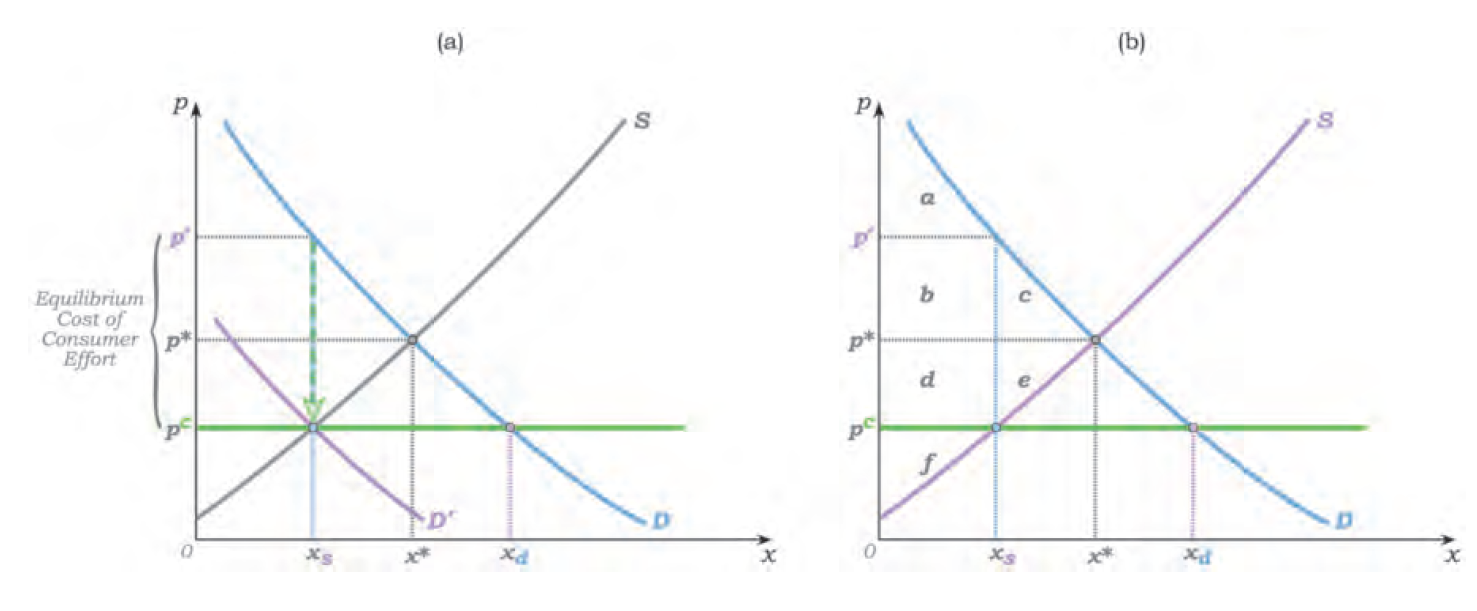
\includegraphics[width=1\textwidth]{18_8} %插入图片,[]中设置图片大小,{}中是图片文件名
	\caption{The Impact of Price Ceilings with Non-Price Rationing} %最终文档中希望显示的图片标题
	\label{Fig.main9} %用于文内引用的标签
\end{figure}

市场若想使所有的经济主体在给定的环境下都努力达到最优化的新的均衡,最初的需求曲线D必须下降到供求均衡的状态。新均衡中每单位额外努力的成本就等于$ (p'-p^c) $。

加入消费者最终将支付的价格是需求曲线$ D' $上的$ p^c $加上努力的成本$ (p'-p^c) $,也就是说消费者最后实际支付的价格为$ p' $。

如果想要得到商品的人利用“副业”(如贿赂)而得到商品,$ (p'-p^c) $的每单位成本对消费者来说是成本,对受贿者来说是收益。这样,消费者的额外成就是经济中其他人的收入,而非无谓损失。但区域$ (c+e) $并不能弥补,因为产生此部分剩余的产品不再被生产了。因此,价格上限所造成的总的无谓损失大小在区域(c+e)到区域(b+c+d+e)之间,这取决于决定新均衡的非价格配给的具体形式。

\hspace*{\fill}

为消除价格上限造成的商品短缺的政府政策

在执行价格上限的情况下,政府通常更可能会执行配给机制来决定有限的商品由谁来获得。无论什么政策都不可能改变一个事实:干预市场价格机制会造成无谓损失。

\hspace*{\fill}

一些价格上限为零的“市场”的伦理思考

器官交易市场的价格上限为零,者造成了器官短缺和很多不必要的死亡。尽管如此,处于伦理考虑,还是将器官市场价格上限设为零。

\hspace*{\fill}

“集中分享收益,分散承担成本”的政治

利益团体可以影响政策制定过程,如果政策的利益集中由少数人获得,那么特定的收益团体会更有效率;如果政策利益过于分散,那么成本会很高。

\subsection{关于一般均衡考虑的一个注解}

这张的价格扭曲政策的分析完全在局部均衡框架内,在局部均衡框架内就明确假定在一个市场执行价格上限和价格下限不会影响其他市场,也就是说其效果没有“溢出”效应。但对政策全面分析就考虑这种溢出效应的话,对政策的影响的分析就会有所不同。

\section{弹性与价格扭曲的数学分析}

\subsection{弹性}

需求价格弹性

\[
\epsilon_d=\frac{dx}{dp}\frac{p}{x(p)}
\]

\hspace*{\fill}

价格弹性和消费者支出

当价格弹性介于0和-1之间时,价格增加会使得消费者支出增加,而当价格弹性小于-1时,价格增加会使消费者支出减少。

假设需求方程是一般的x(p)形式。价格上涨导致的总的消费者支出的变化可以表示为对TS求价格的导数:

\[
\frac{d(TS)}{dp}=x(p)+p\frac{dx}{dp}=x(p)(1+\frac{p}{x}\frac{dx}{dp})=x(p)(1+\epsilon_d)
\]

\hspace*{\fill}

其他类型的价格弹性

需求的收入弹性:

\[
\epsilon_I=\frac{dx}{dI}\frac{I}{x(I)}
\]

交叉价格弹性:

\[
\epsilon_{x_i,p_j}\frac{dx_i}{dp_j}\frac{p_j}{x_i(p_j)}
\]

供给的价格弹性:

\[
\epsilon_s=\frac{dx_s}{dp}\frac{p}{x_s(p)}
\]










\hspace*{\fill}




















	
\end{document}